\documentclass[11pt]{article}

% ---------------------------------------------------------------------------
%  An epigenetic input to the recombination landscape
%  Working draft for discussion — Giles, Ortiz-Barrientos, Saenz-Agudelo
%  Compiles with pdfLaTeX on Overleaf. Upload model_illustration.pdf alongside.
% ---------------------------------------------------------------------------

\usepackage[margin=1in]{geometry}
\usepackage{amsmath, amssymb, amsthm}
\usepackage{graphicx}
\usepackage{booktabs}
\usepackage{microtype}
\usepackage[round,authoryear]{natbib}
\usepackage[hidelinks]{hyperref}
\usepackage{xcolor}

\newtheorem{assumption}{Assumption}
\newtheorem{proposition}{Proposition}
\newtheorem{prediction}{Prediction}
\theoremstyle{remark}
\newtheorem*{remark}{Intuition}

\newcommand{\dd}{\,\mathrm{d}}
\newcommand{\E}{\mathbb{E}}
\newcommand{\avg}[1]{\langle #1 \rangle}

\title{\bfseries An epigenetic input to the recombination landscape\\[6pt]
{\large\normalfont Environmentally induced chromatin accessibility redistributes
crossovers and reshapes genetic diversity}}

\author{
Emily C.\ Giles\,$^{1}$ \and
Daniel Ortiz-Barrientos\,$^{2}$ \and
Pablo Saenz-Agudelo\,$^{1,3}$
}
\date{\today \\[4pt]
\small $^{1}$Cawthron Institute, Nelson, Aotearoa New Zealand \quad
$^{2}$School of the Environment, The University of Queensland \\
\small $^{3}$Instituto de Ciencias Ambientales y Evolutivas, Universidad Austral de Chile \\[2pt]
\small \textit{Working draft for discussion — affiliations to confirm; not for circulation.}}

\begin{document}
\maketitle

\begin{abstract}
\noindent
Invading populations often carry depleted genetic variation yet adapt with
surprising speed --- the \emph{genetic paradox of invasion}. One proposed
ingredient is that heritable epigenetic states supply raw material for the
response. We make a narrow, testable version of that idea precise. Building on
the standard result that meiotic crossovers concentrate in open chromatin in
taxa that lack \textsc{prdm9}, we treat chromatin accessibility as the signal
that \emph{positions} a homeostatically fixed budget of crossovers. A transient,
environmentally induced change in accessibility then \emph{redistributes}
crossovers rather than adding or removing them: we prove the redistribution is
exactly zero-sum, and we give a sign-explicit rule --- a region gains
recombination if and only if it opens by more than the genome-wide average.
Because neutral diversity tracks local recombination under linked selection, the
same perturbation makes diversity \emph{migrate} toward the regions the
environment keeps open. The novelty is not that chromatin gates expression (it
does, and that is textbook); it is that an epigenetic, environmentally set, and
partly heritable input feeds the \emph{genetic} machinery of recombination and
leaves a heritable imprint on the diversity landscape --- an epigenetic cause
with a genetic consequence. We state four falsifiable predictions, separate the
short-term (map) from the long-term (diversity) signatures, and outline a
comparative test across native--invader pairs.
\end{abstract}

\section{Introduction}

Colonising populations need genetic variation to adapt, yet invaders often show
reduced variation; despite this they frequently adapt fast
\citep{sakai2001,perez2006,simberloff2011}. A recurring suggestion is that
heritable epigenetic states, not sequence variation alone, contribute to the
rapid response \citep{nota2023}. Chromatin accessibility --- how reachable a
stretch of DNA is to the proteins that read and recombine it --- is a natural
candidate, because it is environment-sensitive and spatially structured along
the genome \citep{klemm2019}.

The field is careful, and rightly so, about the direction of causation. The
default and well-supported view is that sequence and \emph{trans} factors shape
chromatin, and chromatin acts downstream as a regulator of expression. The bolder
proposition --- the one worth a theory note --- runs partly the other way: that an
epigenetic state can feed back into the \emph{genetic} machinery and reshape the
heritable variation itself. This paper isolates one concrete, mechanistic channel
for that feedback: meiotic recombination. We deliberately recover the standard
result first and add a single increment on top, so that the bolder claim inherits
the credibility of the established one.

The plan is as follows. Section~\ref{sec:model} fixes the baseline: accessibility
positions a fixed budget of crossovers (two recovered results).
Section~\ref{sec:redistribution} introduces the increment: an environmentally
induced change in accessibility redistributes crossovers, zero-sum, with an
explicit sign. Section~\ref{sec:diversity} carries the consequence to neutral
diversity through linked selection, and separates timescales.
Section~\ref{sec:feedback} states the heritability layer that makes the channel a
genuine epigenetic$\,\to\,$genetic feedback. Section~\ref{sec:predictions} lists
falsifiable predictions and a comparative design;
Section~\ref{sec:discussion} states scope and caveats.

\section{A minimal model of accessibility-positioned recombination}
\label{sec:model}

Let $x \in [0, L]$ index position along a chromosome and let $a(x) \ge 0$ be a
measurable accessibility density (an ATAC-seq--type signal), defined in the cells
that undergo meiosis.

\subsection{Recovered result 1: accessibility permits crossover initiation}

Crossovers begin with programmed double-strand breaks (DSBs) cut by \textsc{spo11},
a topoisomerase-like enzyme that must physically reach the DNA; nucleosomes
occlude it. Across taxa the DSB map therefore tracks open chromatin: in budding
yeast the DSB map is essentially the negative of the nucleosome map
\citep{pan2011}, and in \emph{Arabidopsis} crossovers cluster in open,
promoter-proximal regions \citep{choi2013,tock2018}. We encode this as a monotone
relationship between accessibility and DSB intensity,
\begin{equation}
\lambda(x) \;=\; \lambda_0\, f\!\big(a(x)\big), \qquad f' > 0,
\label{eq:dsb}
\end{equation}
and use the linear instance $f(a)=a$ for transparency.

\begin{assumption}[scope: \textsc{prdm9}-free placement]\label{a:prdm9}
In some mammals \textsc{prdm9} overrides the accessibility default, opening
chromatin at sequence motifs and directing DSBs there. \textsc{prdm9} is
lineage-restricted; in taxa that lack it (plants, fungi, birds), placement
reverts to the accessibility default. We assume the focal taxa lack a
\textsc{prdm9}-type director, so that \eqref{eq:dsb} governs placement. For kelp
this is a one-line genomic check --- confirm \textsc{spo11} present and a
\textsc{prdm9}-type director absent --- and we treat it as a precondition, not a
result.
\end{assumption}

\subsection{Recovered result 2: homeostasis fixes the budget, accessibility sets the shape}

Not every DSB becomes a crossover. The number of crossovers per bivalent is
tightly regulated --- at least one obligate crossover, plus interference and
crossover homeostasis that buffer the total against variation in DSB number
\citep{martini2006}. DSBs are in excess; the crossover \emph{count} is the
limiting, conserved quantity. Accessibility therefore sets \emph{where} a fixed
budget of crossovers falls, not \emph{how many}. Writing $A=\int_0^L a(x)\dd x$,
define the normalised placement density and the realised recombination map
\begin{equation}
p(x) \;=\; \frac{a(x)}{A}, \qquad \int_0^L p(x)\dd x = 1, \qquad
r(x) \;=\; R\,p(x), \qquad \int_0^L r(x)\dd x = R,
\label{eq:placement}
\end{equation}
where $R$ is the conserved total recombination set by homeostasis.

\begin{remark}
$p(x)$ answers a biologist's question: ``of the crossovers that \emph{must}
happen, what fraction land here?'' The answer depends only on the \emph{relative}
openness of each region. This normalisation --- nothing more --- is what makes the
next result zero-sum.
\end{remark}

\section{Environmentally induced redistribution of crossovers}
\label{sec:redistribution}

Now let a parental environmental cue (here, heat) perturb accessibility,
\begin{equation}
a(x) \;\longrightarrow\; \tilde a(x) = a(x) + \Delta a(x), \qquad
\tilde A = A + \Delta A, \quad \Delta A = \int_0^L \Delta a(x)\dd x .
\end{equation}
The crossover budget $R$ is unchanged (homeostasis), so the map becomes
$\tilde r(x) = R\,\tilde p(x)$ with $\tilde p = \tilde a / \tilde A$, and the change is
\begin{equation}
\Delta r(x) \;=\; R\big[\tilde p(x) - p(x)\big]
\;=\; R\!\left[\frac{a(x)+\Delta a(x)}{A+\Delta A} - \frac{a(x)}{A}\right].
\label{eq:dr-exact}
\end{equation}

\begin{proposition}[exact zero-sum law]\label{p:zero}
For any perturbation $\Delta a$, the total recombination is conserved and the
redistribution integrates to zero:
\[
\int_0^L \Delta r(x)\dd x
= R\!\left(\int_0^L \tilde p \dd x - \int_0^L p \dd x\right)
= R(1-1) = 0 .
\]
\end{proposition}

\noindent
This holds \emph{exactly}, for perturbations of any size, because $p$ and
$\tilde p$ are both normalised. Heat does not create or destroy recombination; it
moves it. To read \emph{where} it moves, write the perturbation as a local
fractional opening, $\Delta a(x) = a(x)\,g(x)$ with $g = \Delta a / a$, and define
the accessibility-weighted mean opening $\avg{g}_p = \int_0^L p(x)\,g(x)\dd x$
(note $\Delta A / A = \avg{g}_p$). A first-order expansion of \eqref{eq:dr-exact}
gives the interpretable form.

\begin{proposition}[sign-explicit redistribution]\label{p:sign}
To first order in $g$,
\begin{equation}
\boxed{\;\Delta r(x) \;\approx\; R\,p(x)\,\big(g(x) - \avg{g}_p\big)\;}
\label{eq:dr-linear}
\end{equation}
so a region \emph{gains} crossovers iff it opens by more than the genome-wide
average, $g(x) > \avg{g}_p$, and loses them otherwise. The gains and losses
balance: $\int p\,(g-\avg{g}_p)\dd x = \avg{g}_p - \avg{g}_p = 0$, consistent with
Proposition~\ref{p:zero}.
\end{proposition}

\begin{proof}
From \eqref{eq:dr-exact},
$\tilde p = \dfrac{a(1+g)}{A(1+\avg{g}_p)} = p\,\dfrac{1+g}{1+\avg{g}_p}
\approx p(1+g)(1-\avg{g}_p) \approx p\big(1 + g - \avg{g}_p\big)$,
dropping terms of order $g^2$. Hence $\tilde p - p \approx p(g-\avg{g}_p)$, and
multiplying by $R$ gives \eqref{eq:dr-linear}.
\end{proof}

\begin{remark}
This is the formal content of ``\emph{where} recombination is localised,'' not
``recombination decreases.'' A naive reading of an opened region in isolation
would call it more recombinant; the correct, conserved statement is relative ---
opened regions gain at the expense of the rest. The sign turns on a comparison to
the genome-wide mean, which is exactly the quantity a single-locus intuition
omits.
\end{remark}

\section{Consequences for genetic diversity}
\label{sec:diversity}

\subsection{Linked selection ties diversity to local recombination}

Neutral diversity is not uniform: it rises with local recombination rate, the
classical correlation of \citet{begun1992}. Two non-exclusive mechanisms predict
it. Background selection removes linked neutral variation, more severely where
recombination is low \citep{charlesworth1993,hudson1995,nordborg1996}; recurrent
selective sweeps (genetic draft) likewise depress diversity more where
recombination cannot rescue linked sites \citep{maynard1974,stephan1992}. Both
yield a reduction factor $B$ that is increasing in the local map density,
\begin{equation}
\pi(x) \;=\; \pi_0\, B\!\big(r(x)\big), \qquad B' > 0,
\label{eq:pi}
\end{equation}
with $\pi_0$ the diversity expected free of linked selection. (For illustration,
a recurrent-sweep heuristic gives $B(r)\!\propto\![1+\alpha\nu/r]^{-1}$ and
background selection $B(r)=\exp(-V/r)$; both are increasing in $r$.)

\subsection{Diversity migrates toward opened regions}

Linearising \eqref{eq:pi} about the control map and substituting
\eqref{eq:dr-linear},
\begin{equation}
\Delta\pi(x) \;\approx\; \pi_0\, B'\!\big(r(x)\big)\,\Delta r(x)
\;\approx\; \pi_0\, B'\!\big(r(x)\big)\, R\, p(x)\,\big(g(x)-\avg{g}_p\big).
\label{eq:dpi}
\end{equation}
Because $B' > 0$, the sign of $\Delta\pi$ matches the sign of $\Delta r$, hence the
sign of $g(x)-\avg{g}_p$:
\begin{equation}
\operatorname{sign}\Delta\pi(x) \;=\; \operatorname{sign}\big(g(x)-\avg{g}_p\big).
\end{equation}
Diversity rises where the environment opens chromatin more than average, and falls
where recombination was withdrawn. In words: \emph{diversity migrates toward the
regions heat keeps open}. Figure~\ref{fig:model} shows the three results computed
directly from the equations; the redistribution integrates to zero to machine
precision, and the sign rules hold at every informative site.

\begin{figure}[t]
\centering
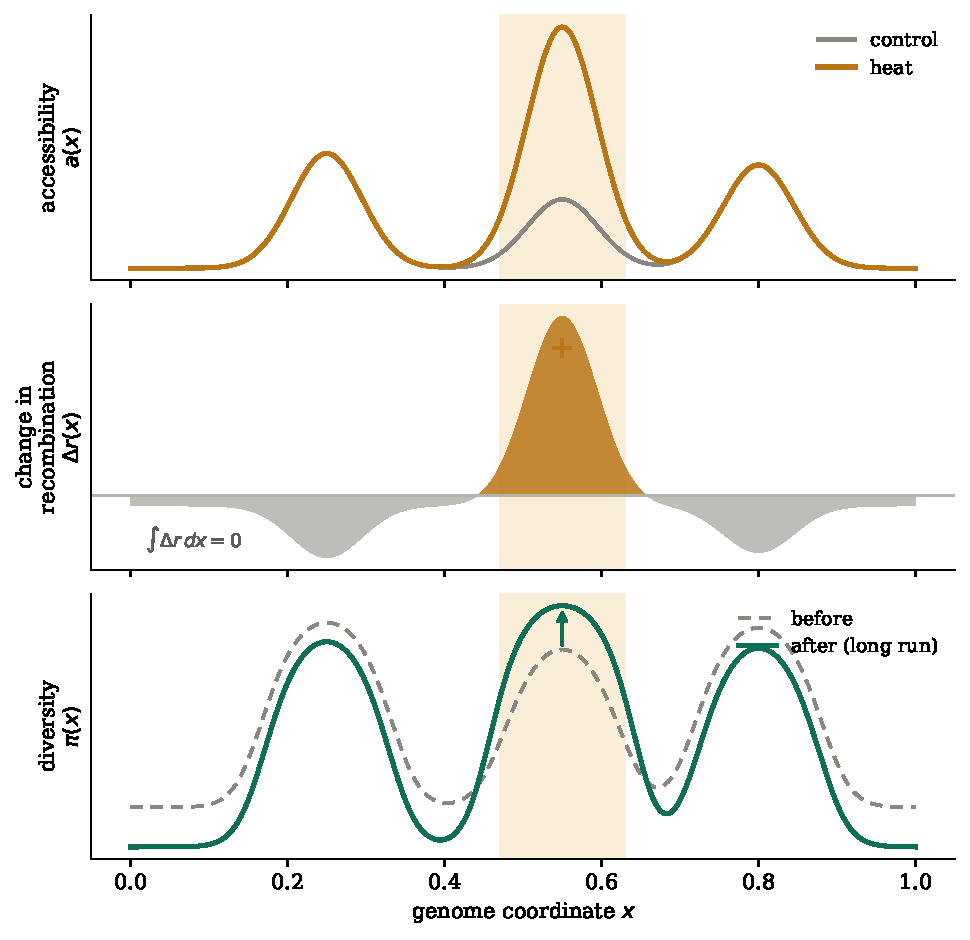
\includegraphics[width=0.78\textwidth]{model_illustration.pdf}
\caption{The model evaluated numerically. \textbf{Top:} control vs.\ heat
accessibility $a(x)$; heat opens the central region (shaded) by more than the
genome-wide average. \textbf{Middle:} the resulting change in the recombination
map $\Delta r(x)$ --- a gain in the opened region ($+$) exactly balanced by losses
elsewhere ($\int\Delta r\dd x = 0$). \textbf{Bottom:} equilibrium neutral
diversity $\pi(x)$ before (dashed) and after (solid); diversity \emph{migrates}
toward the opened region and recedes where recombination was lost. Curves are
computed from Eqs.~\eqref{eq:placement}--\eqref{eq:dpi}; the three internal checks
(zero-sum, $\operatorname{sign}\Delta r$, $\operatorname{sign}\Delta\pi$) pass.}
\label{fig:model}
\end{figure}

\subsection{Two timescales}\label{sec:timescales}

The map change and the diversity change are not simultaneous. The redistribution
$\Delta r$ is immediate: it is present in the meiosis of the exposed generation.
The diversity response $\Delta\pi$ is an \emph{equilibrium} statement of linked
selection and accrues over the relaxation time of diversity, on the order of $N_e$
generations modulated by the local map. This distinction matters for design and
for scope. A parental/intergenerational experiment can detect $\Delta a$ and
$\Delta r$ directly; the diversity imprint $\Delta\pi$ is an evolutionary readout,
visible only if the perturbation is recurrent and sustained --- which is why the
population-genetic signature is best sought comparatively, across populations with
contrasting long-run thermal histories, rather than within a single short
experiment.

\section{Heritability and the epigenetic\,$\to$\,genetic feedback}
\label{sec:feedback}

The results so far would hold even if accessibility reset every generation. The
\emph{novel} claim requires one more ingredient: that the accessibility state is
itself partly heritable, so that a transient cue can leave a persistent mark. Let
$a_t(x)$ be the accessibility in generation $t$, with an environment-set target
$a^\ast(x; E)$ and a transmission coefficient $\rho \in [0,1]$,
\begin{equation}
a_{t+1}(x) \;=\; (1-\rho)\,a^\ast(x; E_t) \;+\; \rho\, a_t(x) \;+\; \xi_t(x),
\label{eq:heritability}
\end{equation}
with $\xi_t$ zero-mean noise. Here $\rho=0$ is pure environmental resetting (no
inheritance) and $\rho>0$ encodes inheritance of the chromatin configuration
across generations. Under a sustained shift in $E$ (a warming regime persisting
$\tau$ generations), \eqref{eq:heritability} relaxes toward an
environment-determined stationary profile, the redistribution $\Delta r$
persists, and --- through Section~\ref{sec:diversity} --- a diversity imprint
$\Delta\pi$ accumulates.

This closes the loop the proposal stakes its novelty on. An epigenetic,
environmentally set, partly heritable input (accessibility) enters the genetic
machinery (recombination) and writes a heritable, sequence-level signature (the
diversity and linkage landscape). The cause is epigenetic; the consequence is
genetic. It does not contradict the orthodox direction of causation --- sequence
and \emph{trans} factors still shape chromatin --- but adds a return channel by
which chromatin state, once set by the environment, reshapes where heritable
variation is exposed and retained. A recurrent epigenetic perturbation thereby
becomes a persistent genetic one.

\begin{remark}[why this matters for the paradox]
Local recombination governs not only neutral diversity but the efficacy of
selection: where recombination is low, Hill--Robertson interference blunts the
response \citep{hillrobertson1966}. Opening a region therefore does two things at
once --- it raises the diversity exposed there and it sharpens selection's grip on
it. An invader with low \emph{genome-wide} variation can, in principle, still
expose and act on useful variation \emph{locally}, in exactly the repeat-rich
reservoirs an environmental cue unlocks. The mechanism does not dissolve the
genetic paradox by itself, but it supplies a concrete route by which depleted
global diversity and rapid local adaptation can coexist.
\end{remark}

\section{Predictions and a comparative test}
\label{sec:predictions}

The chain above is falsifiable at each link. P0 is the recovered base result and
must hold before anything downstream is trusted.

\begin{prediction}[baseline]
In control meiocytes, crossover density correlates positively with accessibility,
after controlling for gene density. \emph{Refuted by} absence of, or a negative,
correlation --- the pathway fails at its base.
\end{prediction}
\begin{prediction}[causal modulation]
Between control and heat, the change in crossover placement co-localises with the
change in accessibility, following \eqref{eq:dr-linear}: regions opening more than
the genome-wide average gain crossovers. \emph{Refuted by} $\Delta r$ and
$g-\avg{g}_p$ being spatially uncorrelated.
\end{prediction}
\begin{prediction}[homeostasis / zero-sum]
Total map length is conserved across treatments while its distribution shifts
($\int\Delta r \approx 0$). \emph{Refuted by} a change in total recombination
without redistribution.
\end{prediction}
\begin{prediction}[diversity imprint]
Across populations or lineages whose thermal histories repeatedly open the same
regions, those regions carry elevated $\pi$ and reduced linkage disequilibrium
consistent with locally elevated recombination, with sign matching
$g-\avg{g}_p$. \emph{Refuted by} opened regions showing no long-run diversity
signature.
\end{prediction}

P0--P2 are reachable within a single experimental programme. P3 is evolutionary
and slow; it is best tested comparatively, ideally across three or more
native--invader (or ancestral--derived) pairs, providing ecological and
evolutionary replication of the same prediction. The two routes are complementary:
the experiment supplies the mechanism ($\Delta a \to \Delta r$), the comparison
supplies the long-run consequence ($\Delta r \to \Delta\pi$), and a simulation
that feeds an empirically measured $\Delta r(x)$ forward can predict the
$\Delta\pi(x)$ a real population would take many generations to reveal.

\section{Scope, caveats, and connections}
\label{sec:discussion}

\paragraph{Necessary, not sufficient.} Open chromatin permits a DSB; it does not
compel one. Axis proteins, cohesin, and marks such as H3K4me3 also gate
initiation, so accessibility \emph{bounds and biases} the crossover map rather
than determining it pointwise. Predictions are therefore framed as controlled
correlations and sign tests, not deterministic laws --- which is the honest and
the sturdier posture.

\paragraph{Where recombination happens.} Recombination is a meiocyte (sporophyte)
event; offspring tissue only records its products. The accessibility relevant to
P0--P2 is that of the sporogenous tissue. Accessibility measured in offspring
answers a \emph{different} question --- whether the state is heritable
(\eqref{eq:heritability}, $\rho>0$) --- and becomes a valid proxy for the meiocyte
state only once that link is shown, not assumed.

\paragraph{Parental, not (yet) transgenerational.} When a stressed parent's
germline is directly exposed, the offspring response is a parental /
intergenerational effect, not transgenerational inheritance, which requires a
further generation with the stressor withdrawn. The heritability layer
\eqref{eq:heritability} is what an unstressed $F_2$ would test; $\rho$ is
estimable only with that design.

\paragraph{Homeostasis is an idealisation.} If the crossover budget is only
partially buffered, $R$ varies and the zero-sum law weakens to approximate
conservation; Proposition~\ref{p:sign} then carries an additional term in
$\Delta R$. The qualitative prediction (redistribution toward above-average
openings) survives as long as homeostasis dominates.

\paragraph{An independent line of evidence.} The directional prediction of
Section~\ref{sec:diversity} --- a consistent, repeatable shift in the
recombination landscape associated with adaptation --- can be sought in parallel
ecotype systems, by asking whether derived ecotypes show a consistent
ancestral$\,\to\,$derived change in recombination, and only then which mechanisms
(inversions, haploblocks, accessibility evolution) drive it. That route needs no
parental experiment and offers a second, population-genetic test of the same idea.

\paragraph{Summary.} The contribution is a single, sign-explicit channel by which
an environmentally induced, partly heritable epigenetic state reshapes the genetic
recombination landscape and, through linked selection, the diversity landscape. We
recovered the established result (accessibility positions crossovers) before
adding the increment (heat redistributes them, zero-sum) and its consequence
(diversity migrates), and we kept the bolder, feedback claim falsifiable at every
step.

\bibliographystyle{plainnat}
\begin{thebibliography}{99}
\small

\bibitem[Begun \& Aquadro(1992)]{begun1992}
Begun DJ, Aquadro CF. 1992. Levels of naturally occurring DNA polymorphism
correlate with recombination rates in \emph{D.\ melanogaster}.
\emph{Nature} 356:519--520.

\bibitem[Charlesworth et al.(1993)]{charlesworth1993}
Charlesworth B, Morgan MT, Charlesworth D. 1993. The effect of deleterious
mutations on neutral molecular variation. \emph{Genetics} 134:1289--1303.

\bibitem[Choi et al.(2013)]{choi2013}
Choi K, Zhao X, Kelly KA, et al. 2013. \emph{Arabidopsis} meiotic crossover hot
spots overlap with H2A.Z nucleosomes at gene promoters.
\emph{Nature Genetics} 45:1327--1336.

\bibitem[Hill \& Robertson(1966)]{hillrobertson1966}
Hill WG, Robertson A. 1966. The effect of linkage on limits to artificial
selection. \emph{Genetical Research} 8:269--294.

\bibitem[Hudson \& Kaplan(1995)]{hudson1995}
Hudson RR, Kaplan NL. 1995. Deleterious background selection with recombination.
\emph{Genetics} 141:1605--1617.

\bibitem[Klemm et al.(2019)]{klemm2019}
Klemm SL, Shipony Z, Greenleaf WJ. 2019. Chromatin accessibility and the
regulatory epigenome. \emph{Nature Reviews Genetics} 20:207--220.

\bibitem[Martini et al.(2006)]{martini2006}
Martini E, Diaz RL, Hunter N, Keeney S. 2006. Crossover homeostasis in yeast
meiosis. \emph{Cell} 126:285--295.

\bibitem[Maynard Smith \& Haigh(1974)]{maynard1974}
Maynard Smith J, Haigh J. 1974. The hitch-hiking effect of a favourable gene.
\emph{Genetical Research} 23:23--35.

\bibitem[Nordborg et al.(1996)]{nordborg1996}
Nordborg M, Charlesworth B, Charlesworth D. 1996. The effect of recombination on
background selection. \emph{Genetical Research} 67:159--174.

\bibitem[Nota et al.(2023)]{nota2023}
Nota A, Bertolino S, Tiralongo F, Santovito A. 2023. Adaptation to bioinvasions:
when does it occur? \emph{Global Change Biology} 29:5891--5908.

\bibitem[Pan et al.(2011)]{pan2011}
Pan J, Sasaki M, Kniewel R, et al. 2011. A hierarchical combination of factors
shapes the genome-wide topography of yeast meiotic recombination initiation.
\emph{Cell} 144:719--731.

\bibitem[Perez et al.(2006)]{perez2006}
Perez JE, Nirchio M, Alfonsi C, Munoz C. 2006. The biology of invasions: the
genetic adaptation paradox. \emph{Biological Invasions} 8:1115--1121.

\bibitem[Sakai et al.(2001)]{sakai2001}
Sakai AK, Allendorf FW, Holt JS, et al. 2001. The population biology of invasive
species. \emph{Annual Review of Ecology and Systematics} 32:305--332.

\bibitem[Simberloff \& Rejm\'anek(2011)]{simberloff2011}
Simberloff D, Rejm\'anek M (eds). 2011. \emph{Encyclopedia of Biological
Invasions}. University of California Press.

\bibitem[Stephan et al.(1992)]{stephan1992}
Stephan W, Wiehe THE, Lenz MW. 1992. The effect of strongly selected
substitutions on neutral polymorphism. \emph{Theoretical Population Biology}
41:237--254.

\bibitem[Tock \& Henderson(2018)]{tock2018}
Tock AJ, Henderson IR. 2018. Hotspots for initiation of meiotic recombination.
\emph{Frontiers in Genetics} 9:521.

\end{thebibliography}

\end{document}
